\documentclass[
	10pt, % Set the default font size, options include: 8pt, 9pt, 10pt, 11pt, 12pt, 14pt, 17pt, 20pt
	%t, % Uncomment to vertically align all slide content to the top of the slide, rather than the default centered
	aspectratio=169, % Uncomment to set the aspect ratio to a 16:9 ratio which matches the aspect ratio of 1080p and 4K screens and projectors
	% table,
]{beamer}

\graphicspath{{figures/}{./}} % Specifies where to look for included images (trailing slash required)

\usepackage{booktabs} % Allows the use of \toprule, \midrule and \bottomrule for better rules in tables

\usetheme{rpi}
\addbibresource{references.bib}
%----------------------------------------------------------------------------------------
% PRESENTATION INFORMATION
%----------------------------------------------------------------------------------------

% \title[A Short Title for Your Slides]{A Very Long and Multi-Lined Full Presentation Title That You Probably Shouldn't Use Because Titles Should not be This Long, but I Will Do It For Debugging} 
\title[A Short Title for Your Slides]{(Unofficial)\\RPI Beamer Presentation Template}
\subtitle{Optional Subtitle} % Presentation subtitle, remove this command if a subtitle isn't required
\author[]{Inwon Kang \and StackOverflow} % Presenter name(s), the optional parameter can contain a shortened version to appear on the bottom of every slide, while the main parameter will appear on the title slide
\institute[RPI]{Department of Computer Science}

\date[\today]{\today}

% NOTE: Comment this out if you don't want it
\AtBeginSection[]{
	\begin{frame}[noframenumbering]
		\frametitle{Outline}
		\begin{columns}[t]
			\begin{column}{.05\textwidth}\end{column}
			\begin{column}{.45\textwidth}
				\tableofcontents[
					currentsection,
					% sectionstyle=show/hide,
					subsectionstyle=hide/show/hide,
					sections={-3},
				]
			\end{column}
			\begin{column}{.45\textwidth}
				\tableofcontents[
					currentsection,
					% sectionstyle=show/hide,
					subsectionstyle=hide/show/hide,
					sections={4-},
				]
			\end{column}
		\end{columns}
		% NOTE: If you don't want them to affect the slide number
		% \addtocounter{framenumber}{-1}
	\end{frame}
}

% NOTE: Comment this out if you don't want it
\AtBeginSubsection[]{
	\begin{frame}[noframenumbering]
		\frametitle{Outline}
		\begin{columns}[t]
			\begin{column}{.05\textwidth}
			\end{column}
			\begin{column}{.45\textwidth}
				\tableofcontents[
					currentsection,
					currentsubsection,
					% sectionstyle=show/hide,
					% subsectionstyle=show/hide,
					sections={-3},
				]
			\end{column}
			\begin{column}{.45\textwidth}
				\tableofcontents[
					currentsection,
					currentsubsection,
					% sectionstyle=show/hide,
					% subsectionstyle=show/hide,
					sections={4-},
				]
			\end{column}
		\end{columns}
	\end{frame}
}

\begin{document}
% NOTE: Plain is what blocks the footline from showing up on the title page
\begin{frame}[plain]
	\titlepage % Output the title slide, automatically created using the text entered in the PRESENTATION INFORMATION block above
\end{frame}

%----------------------------------------------------------------------------------------
% TABLE OF CONTENTS SLIDE
%----------------------------------------------------------------------------------------

% The table of contents outputs the sections and subsections that appear in your presentation, specified with the standard \section and \subsection commands. You may either display all sections and subsections on one slide with \tableofcontents, or display each section at a time on subsequent slides with \tableofcontents[pausesections]. The latter is useful if you want to step through each section and mention what you will discuss.

\begin{frame}[noframenumbering]
	\frametitle{Presentation Overview} % Slide title, remove this command for no title

	% NOTE: Two column version
	\begin{columns}[t]
		\begin{column}{.05\textwidth}
		\end{column}
		\begin{column}{.45\textwidth}
			\tableofcontents[
				pausesections,
				sections={-3}
			]
		\end{column}
		\begin{column}<+->{.45\textwidth}
			\only<.>{\setcounter{tocseccounter}{\slideinframe}}
			\advanceslidecounter{-\thetocseccounter}
			\tableofcontents[
				pausesections,
				sections={4-}
			]
		\end{column}
	\end{columns}

	% NOTE: One column version
	%\tableofcontents[pausesections] % Output the table of contents (break sections up across separate slides)
\end{frame}

%----------------------------------------------------------------------------------------
% Actual Contents
%----------------------------------------------------------------------------------------

\section{Introduction}
\begin{frame}
	\frametitle{Introduction} % Slide title, remove this command for no title
	\framesubtitle{A subtitle}
	{
		\Large \bf
		What is this?
	}

	A template for beamer presentations.
	I made this template following RPI's official powerpoint template and logos~\cite{rpiHomeStrategicCommunications}.

	\vspace{1cm}
	{
		\Large \bf
		Why did I do this?
	}

	I couldn't find an existing one and I didn't want to copy over citations manually.

\end{frame}

\begin{frame}{Before We Start}
	\begin{itemize}
		\item This project uses the \texttt{fontspec} package, which is not supported by the default compiler backend on Overleaf.
		\item You can change this by following the two steps:
	\end{itemize}
	\begin{minipage}[t]{0.48\textwidth}
		\begin{figure}
			\begin{center}
				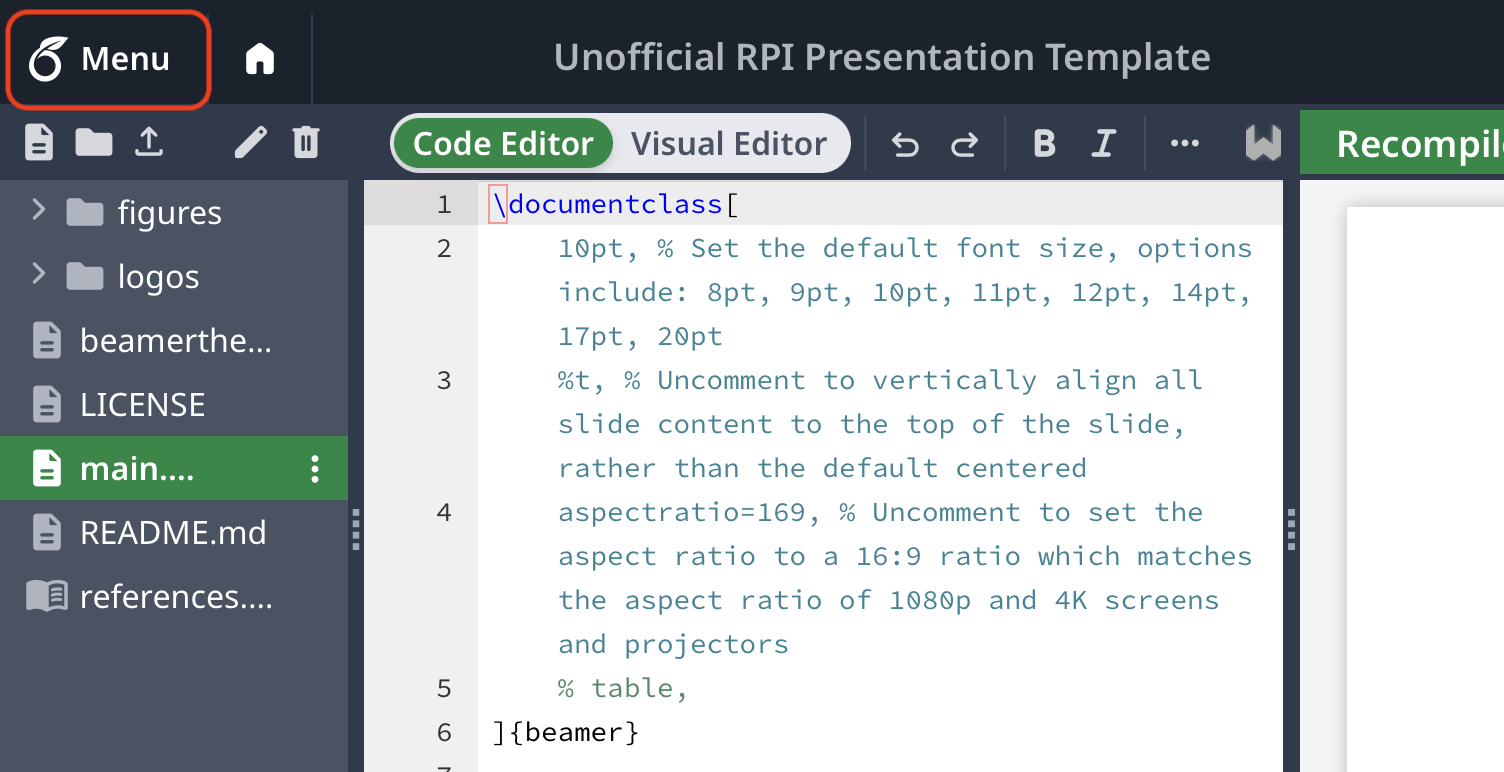
\includegraphics[width=0.95\textwidth]{figures/overleaf-menu.png}
			\end{center}
			\caption{Open the menu tab}\label{fig:overleaf-menu}
		\end{figure}
	\end{minipage}%
	\begin{minipage}[t]{0.48\textwidth}
		\begin{figure}
			\begin{center}
				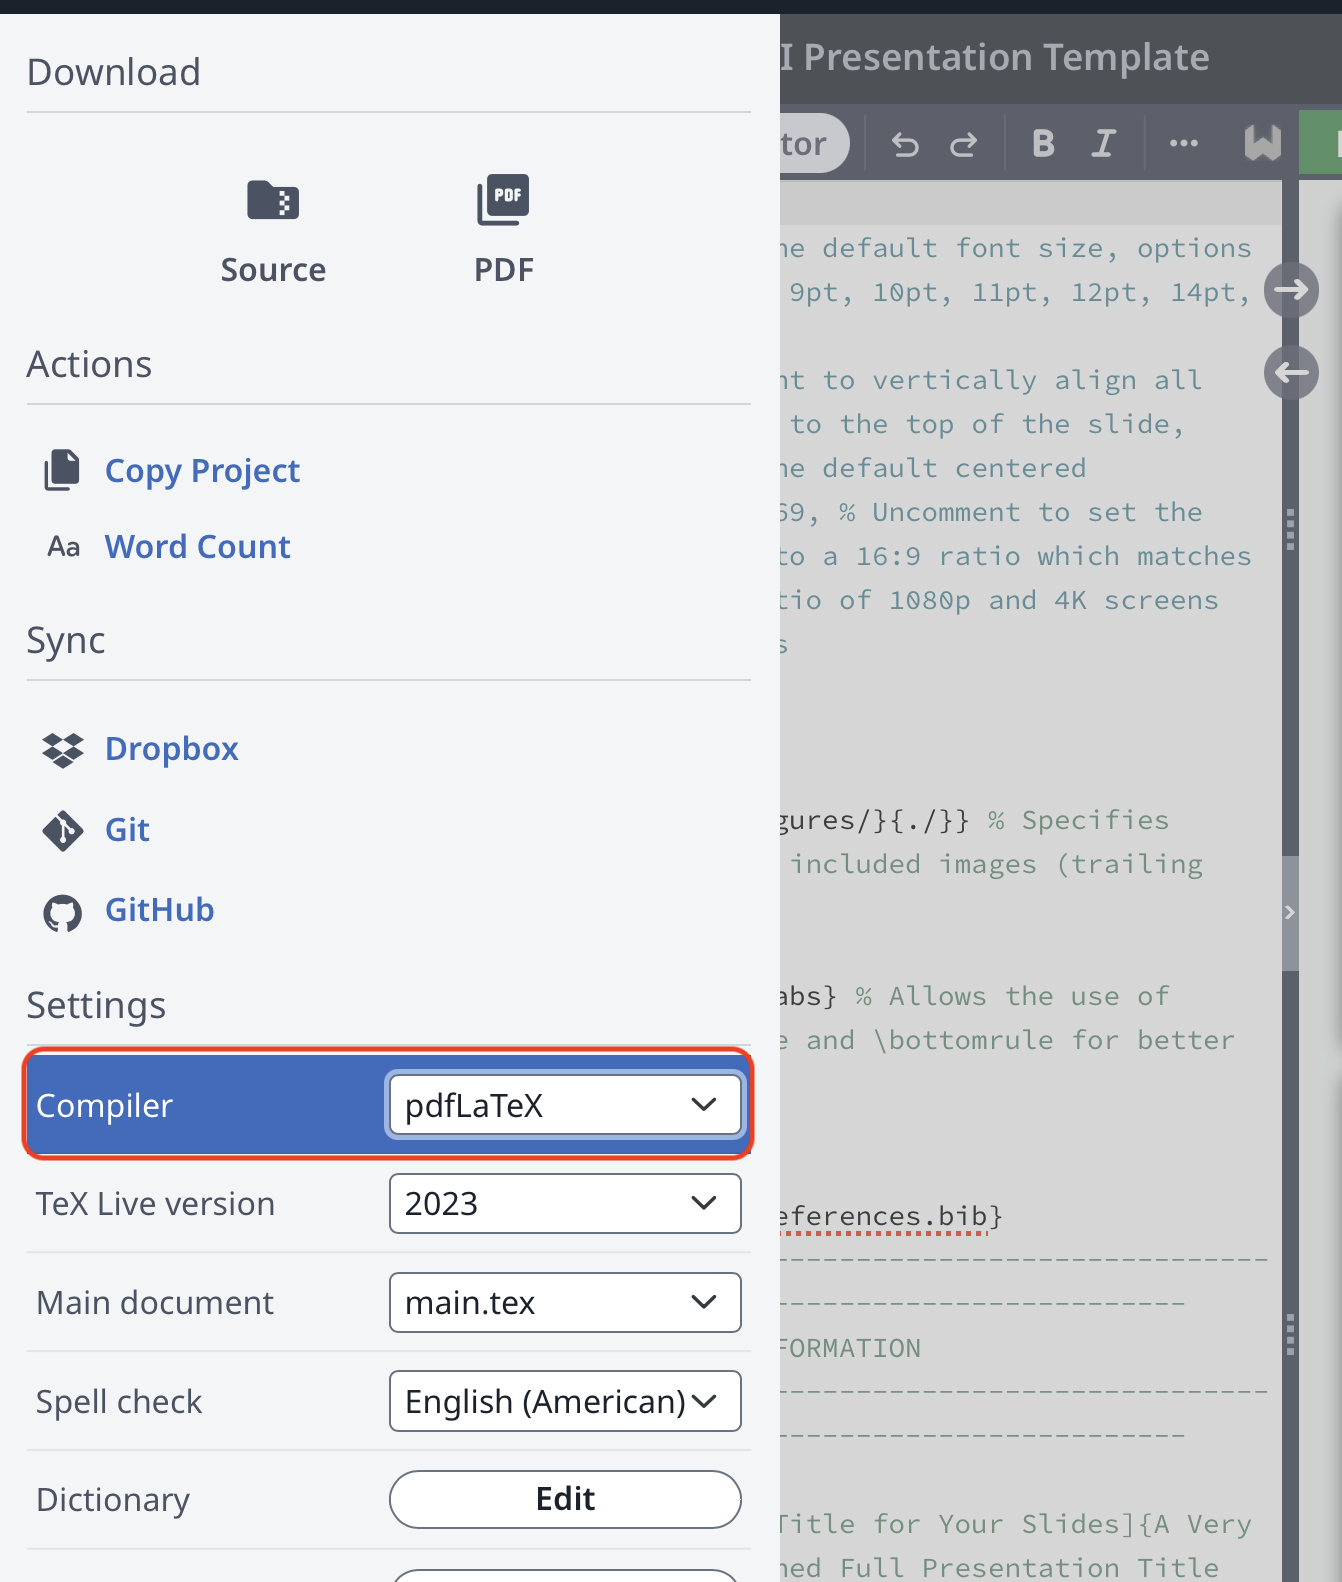
\includegraphics[width=0.4\textwidth]{figures/overleaf-compiler.png}
			\end{center}
			\caption{Set compiler to XeLaTex}\label{fig:overleaf-compiler}
		\end{figure}
	\end{minipage}%
\end{frame}

\begin{frame}{Style Notes}
	\begin{itemize}
		\item Use of \texttt{minipage} is encouraged.
		      \begin{itemize}
			      \item Why? because I designed the template with it in mind. The columns env probably works for the most part as well, but it might not.
		      \end{itemize}
		\item I tried to use relative values for margins and header/sizes where I could. It should scale well with different page sizes.
	\end{itemize}
\end{frame}


\section{Table of Contents}
\begin{frame}
	\frametitle{Table of Contents}
	\begin{itemize}
		\item You already saw the table of contents.
		\item By default, it is in one column. If you want to divide it to multiple columns, you can use minipage or columns~\cite{samcarter_is_at_topanswers.xyzAnswerBeamerVertical2013}
		\item To make use of this, you need to use sections, which should be placed outside of the frame~\cite{campaAnswerAtbeginsectionReturns2022}.
		\item Use \texttt{AtBeginSection} to automatically show the table of contents at the beginning of each section.
	\end{itemize}
\end{frame}


\section{List/Figure/Table/Definition}
\subsection{Lists}
\begin{frame}
	\frametitle{Using lists}
	Simple example of using lists.
	\begin{itemize}
		\item Item 1.
		\item Item 2.
	\end{itemize}

	\begin{enumerate}
		\setlength{\leftmargini}{12pt}
		\item Enumerate 1
		\item Enumerate 2
	\end{enumerate}
	I think this looks pretty similar to how the powerpoint one looks.
\end{frame}

\subsection{Figures}
\begin{frame}
	\frametitle{Using figures}
	Here is an example of a figure.
	\begin{figure}
		\centering
		\begin{minipage}{.5\textwidth}
			\centering
			\includegraphics[width=.7\linewidth]{example-image-a}
			\caption{A subfigure}
		\end{minipage}%
		\begin{minipage}{.5\textwidth}
			\centering
			\includegraphics[width=.7\linewidth]{example-image-b}
			\caption{Another subfigure}
		\end{minipage}
		\caption{Example of a figure side by side.}
	\end{figure}
\end{frame}

\subsection{Figures in Full Screen}
\begin{frame}
	\frametitle{Using a full screen image}
	Next slide shows how to use an image in full screen.
	I got this from
	\href{
		https://tex.stackexchange.com/questions/3915/image-on-full-slide-in-beamer-package
	}{\color{RPIred}\underline{here}}
\end{frame}

{
\usebackgroundtemplate{\includegraphics[width=\paperwidth,height=\paperheight]{example-image-a}}
\begin{frame}[plain]
\end{frame}
}

\subsection{Tables}
\begin{frame}
	\frametitle{A Table}
	\centering
	\begin{minipage}{0.3\linewidth}
		\begin{table}
			\centering
			{\small
				\begin{tabular}[c]{lll}
					\toprule
					\textbf{Col 1} & \textbf{Col 2} & \textbf{Col 3} \\ \midrule
					a              & b              & c              \\
					d              & e              & f              \\
					\bottomrule
				\end{tabular}
			}
			\caption{An example table}
			\label{tab:}
		\end{table}
	\end{minipage}
	\begin{minipage}{0.6\linewidth}
		\textbf{Findings}\par
		\begin{itemize}
			\item This is indeed a table.
			\item Use minipage to put two things side by side, just like the images.
			\item You can also use columns, but it's not necessary~\cite{scharrerAnswerMinipageColumns2011}.
		\end{itemize}
	\end{minipage}
\end{frame}

\subsection{Textboxes}
\begin{frame}
	\frametitle{Textboxes}
	\centering
	\begin{minipage}{0.3\linewidth}
		\begin{primaryblock}[equal height group=A,label=block:first]{First Block}
			% I'm also going to set the indent for them so they play nicely with the textboxes
			\setlength{\leftmargini}{8pt}
			\begin{itemize}
				\item First item of first block.
				\item Second item of first block.
				\item Notice that the next block matches the height of this one.
				\item I am also changing the indentation of bullets so it looks better in the boxes.
			\end{itemize}
		\end{primaryblock}
	\end{minipage}
	\begin{minipage}{0.3\linewidth}
		\begin{secondaryblock}[equal height group=A]{Second Block}
			\setlength{\leftmargini}{8pt}
			\begin{itemize}
				\item First item of second block.
				      \begin{itemize}
					      \item first sub item of second block.
				      \end{itemize}
			\end{itemize}
		\end{secondaryblock}
	\end{minipage}
	\begin{minipage}{0.3\linewidth}
		\begin{primaryblock}[]{Third Block}
			% \item First point of second block.
			This one doesn't have a list and doesn't match the height!
		\end{primaryblock}
	\end{minipage}
\end{frame}

\section{Theorem/Definition/Algorithms}

\subsection{Definitions}
\begin{frame}{Definitions}
	\begin{definition}{A definition}
		This is a definition.
		\begin{itemize}
			\item It can be used to define something.
			\item It can also be used to define something else.
			\item If you don't like the colors, you can change \texttt{block title} and  \texttt{block body} of \texttt{setbeamercolor} in the \texttt{.sty} file.\end{itemize}
	\end{definition}
\end{frame}



\section{Using Bibtex}
\begin{frame}
	\frametitle{Using Bibtex}
	\begin{itemize}
		\item It should be the same as using your regular bibtex.
		\item To showcase, let's cite some resources~\cite{anglimAnswerImageFull2010,fiandrinoAnswerDesignCustom2013,kormyloAnswerMakeTikz2017} that helped me put this together.
		\item You can add \texttt{[allowframebreaks]} to the frame to automatically continue the reference list in the text page if you have too many.
		\item You can use \texttt{\textbackslash tcite} (short for textcite) shorthand to use it in \textit{text} mode, i.e. \tcite{anglimAnswerImageFull2010}.
		\item You can use \texttt{\textbackslash fcite} (short for footcite) to add a citation with a footnote on the bottom of the slide.
		      \begin{itemize}
			      \item Note that if you are using \texttt{\textbackslash columns} or \texttt{\textbackslash minipage}, the footnote will by default appear in the bottom of the \textit{environment}, not the slide.
			      \item You can manually escape this by using just \texttt{\textbackslash cite} or \texttt{\textbackslash tcite} in text and adding a \texttt{\textbackslash bfcite} (blank footcite) outside of these environments.
			      \item e.g. \texttt{\textbackslash bfcite\{fiandrinoAnswerDesignCustom2013\}}.
		      \end{itemize}
	\end{itemize}
	\bfcite{fiandrinoAnswerDesignCustom2013}
\end{frame}

\begin{frame}[allowframebreaks]
	\frametitle{References}
	\printbibliography
\end{frame}

\end{document}
